\section{Vorbereitung}

\noindent{\large Arbeitsaufteilung:\par}
\begin{table}[htb]
\centering
\caption{Arbeitsaufteilung in der Gruppe}
\label{Arbeitsaufteilung}
\begin{tabular}{c|ccc}
\toprule
Aufgabe & Lucas & Aleksandra & Timo\\
\midrule
Motivation &  & x & \\
Literaturrecherche &  &  & x\\
1.2 Filterschaltungen & x & x & x\\
1.3 Addierschaltung & x & x & x\\
Dokumentation & x & x & x\\
Diskussionen & x & x & x\\
Bericht \& Spice & x &  & \\
\bottomrule
\end{tabular}
\end{table}

\noindent{\large Genutzte Materialien:\par}
\begin{table}[htb]
\centering
\caption{Genutzte Materialien}
\label{Arbeitsaufteilung}
\begin{tabular}{c|c|c}
\toprule
Bauteiltyp & Beschreibung & Wert\\
\midrule
Digital-Analog-Wandler & MCP4922, 1x & \\
\hline
Operationsverstärker & MCP6002, 4x & \\
\hline
Kondensatoren & 
\vtop{
\hbox{\strut Keramik- und}
\hbox{\strut Elektrolytkondensatoren,}
\hbox{\strut bis 100 nF: 10\% Toleranz,}
\hbox{\strut ab 470 nF: 20\% Toleranz,}
\hbox{\strut 4x oder 2x}
}
& 
\vtop{
\hbox{\strut diverse:}
\hbox{\strut ~~~~10 nF, 22 nF, 33 nF}
\hbox{\strut ~~~~47 nF, 68 nF, 100 nF}
\hbox{\strut ~~~~470 nF, 10 $\mu$F, 100 $\mu$F}
}
\\
\hline
Widerstände &
\vtop{
\hbox{\strut Kohleschichtwiderstände,}
\hbox{\strut 1/4 W,}
\hbox{\strut 5\% Toleranz,}
\hbox{\strut jeweils 10x}
}
& 
\vtop{
\hbox{\strut E6-Reihe:}
\hbox{\strut ~~~~100$\Omega$, 220$\Omega$, 470$\Omega$}
\hbox{\strut ~~~~1 k$\Omega$, 1,5 k$\Omega$, 2,2 k$\Omega$}
\hbox{\strut ~~~~3,3 k$\Omega$, 4,7 k$\Omega$, 6,8 k$\Omega$}
\hbox{\strut ~~~~10 k$\Omega$, 15 k$\Omega$, 22 k$\Omega$}
\hbox{\strut ~~~~33 k$\Omega$, 47 k$\Omega$, 68 k$\Omega$}
\hbox{\strut ~~~~100 k$\Omega$, 220 k$\Omega$, 1 M$\Omega$}
}
\\
\hline
Potentiometer & Potentiometer, 2x & 0...100 k$\Omega$\\
\bottomrule
\end{tabular}
\end{table}

\clearpage
\section{Einleitung}

\subsection{Motivation}

\subsection{Literaturrecherche}


\clearpage
\section{Aufgaben}

\subsection{Filterschaltungen}

\subsubsection{Materialien \& Methoden}

\begin{figure}[htb]
    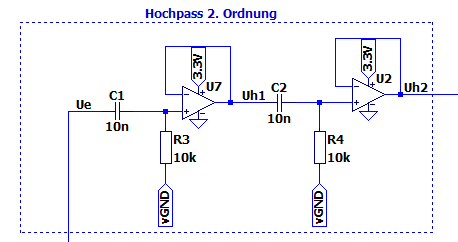
\includegraphics[width=16cm]{./pictures/Hochpass}
    \caption{Aufbau des Hochpasses}
    \label{fig:Hochpass}
\end{figure}

In der Aufgabenstellung wird ein Hochpass der Ordnung zwei gefordert. Diese Anforderung realisieren wir mittels zwei typischer RC-Höchpässe. Diese sind über einen Spannungsfolger gekoppelt. Der gesamte Hochpass ist mit einem weiteren Spannungsfolger vom weiteren Verlauf der Schaltung sicher in Hinsicht auf Rückkopplungen und unzulässiger Ströme abgetrennt.
\\
Um die Kondensatoren und die Widerstände zu dimensionieren, betrachten wir die Frequenzen des Sprachbereiches. Nach diesem Bereich richtet sich dann unsere Grenzfrequenz. Aus der Abbildung der Aufgabenstellung ergibt sich für den Hauptsprachbereich bei normalem Gespräch ein Frequenzbereich von ca. 175Hz - 4000Hz. Unsere angestrebte Frequenz liegt daher in der Mitte bei ca. 1600Hz. Bei der Dimensionierung ergeben sich zwei Unbekannte (Widerstand und Kondensator). Dabei wählen wir für den Kondensator 10nF, da unsere Anzahl an Kondensatoren begrenzt ist und wir weitaus mehr Widerstände besitzen und diese durch geschickte Kombination variieren können. Für die Grenzfrequenz gilt folgende Formel mit $\omega = 2\cdot \pi \cdot f$: 
\gleichung{\omega=\frac{1}{R\cdot C}}{}

\newpage
\gleichung{f=\frac{1}{2\cdot \pi \cdot C \cdot R}}{}

Wir wählen für den Wert unserer Widerstände daher $10k\Omega$. Mit den 10nF der Kondensatoren ergibt sich eine Grenzfrequenz von $1591.6Hz$, welche unserem angestrebten Wert fast entspricht. Die Abweichung von 8.4Hz liegt im Toleranzbereich.
\\
\\
Die Übertragungsfunktion ergibt sich aus der Spannungsteilerregel und dem Verhältnis $U_{h2}$ zu $U_{e}$:
\gleichung{
\begin{split}
&\frac{U_a}{U_e} = \frac{R}{((C+R)||R)+C}
\\
&C+R = \frac{1}{j \omega C}+R = R-j \frac{1}{\omega C}
\\
&(C+R)||R = \frac{R(R-j \frac{1}{\omega C})}{(R-j \frac{1}{\omega C})+(R+j \frac{1}{\omega C})} = \frac{R^2-j \frac{R}{\omega C}}{2R-j \frac{1}{\omega C}}
\end{split}
}{}
\gleichung{
\begin{split}
((C+R)||R)+C &= \frac{R^2-j \frac{R}{\omega C}}{2R-j \frac{1}{\omega C}}+\frac{1}{j \omega C}
\\
&= \frac{R^2-j \frac{R}{\omega C}}{2R-j \frac{1}{\omega C}}-j \frac{1}{\omega C}
\\
&= \frac{(R^2-j \frac{R}{\omega C})(2R-j \frac{1}{\omega C})}{4R^2+\frac{1}{(\omega C)^2}}-j \frac{1}{\omega C}
\\
&= \frac{2R^3+j \frac{R^2}{\omega C}-j \frac{2R^2}{\omega C}+\frac{R}{(\omega C)^2}}{4R^2+\frac{1}{(\omega C)^2}}-j \frac{1}{\omega C}
\\
&= \frac{2R^3-j \frac{R^2}{\omega C}+\frac{R}{(\omega C)^2}}{4R^2+\frac{1}{(\omega C)^2}}-j \frac{1}{\omega C}
\\
\end{split}
}{}
\gleichung{
U_{a}(f)= \left(\frac{2R^3-j \frac{R^2}{\omega C}+\frac{R}{(\omega C)^2}}{4R^2+\frac{1}{(\omega C)^2}}-j \frac{1}{\omega C}\right) \cdot U_{e}(f)
}{}

\newpage
\begin{figure}[htb]
    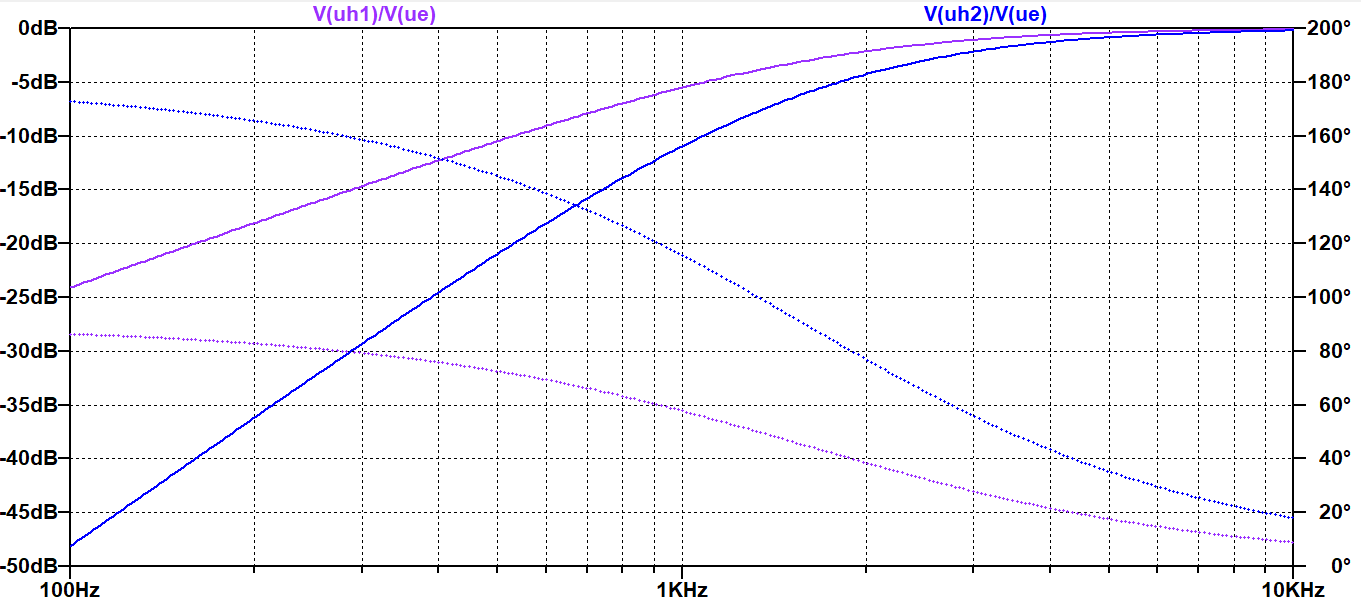
\includegraphics[width=16cm]{./pictures/Hochpass_Bode}
    \caption{Bodediagram des Hochpasses}
    \label{fig:HochpassBode}
\end{figure}

\begin{figure}[htb]
    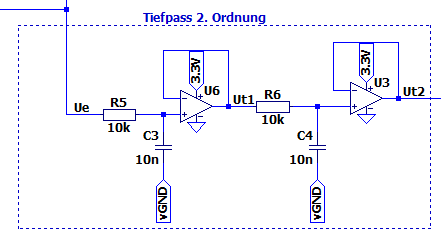
\includegraphics[width=16cm]{./pictures/Tiefpass}
    \caption{Aufbau des Tiefpasses}
    \label{fig:Tiefpass}
\end{figure}

In der Aufgabenstellung wird zudem ein Tiefpass der Ordnung zwei gefordert. Diese Anforderung realisieren wir mittels zwei typischer RC-Tiefpässe. Diese sind über einen Spannungsfolger gekoppelt. Der gesamte Tiefpass ist mit einem weiteren Spannungsfolger vom weiteren Verlauf der Schaltung sicher in Hinsicht auf Rückkopplungen und unzulässiger Ströme abgetrennt.
\\
\\
Wir wählen für unsere Kondensatoren und Widerstände die analogen Werte zum Hochpass, da wir die selbe Grenzfrequenz anstreben und die Frequenzformel des Hochpasses analog für den Tiefpass gilt. Somit erhalten wir auch hier eine Grenzfrequenz von $1591.6Hz$.
\\
\\
Die Übertragungsfunktion ergibt sich gleichermaßen aus der Spannungsteilerregel und dem Verhältnis $U_{t2}$ zu $U_{e}$:
\\
\\
\\
\begin{figure}[htb]
    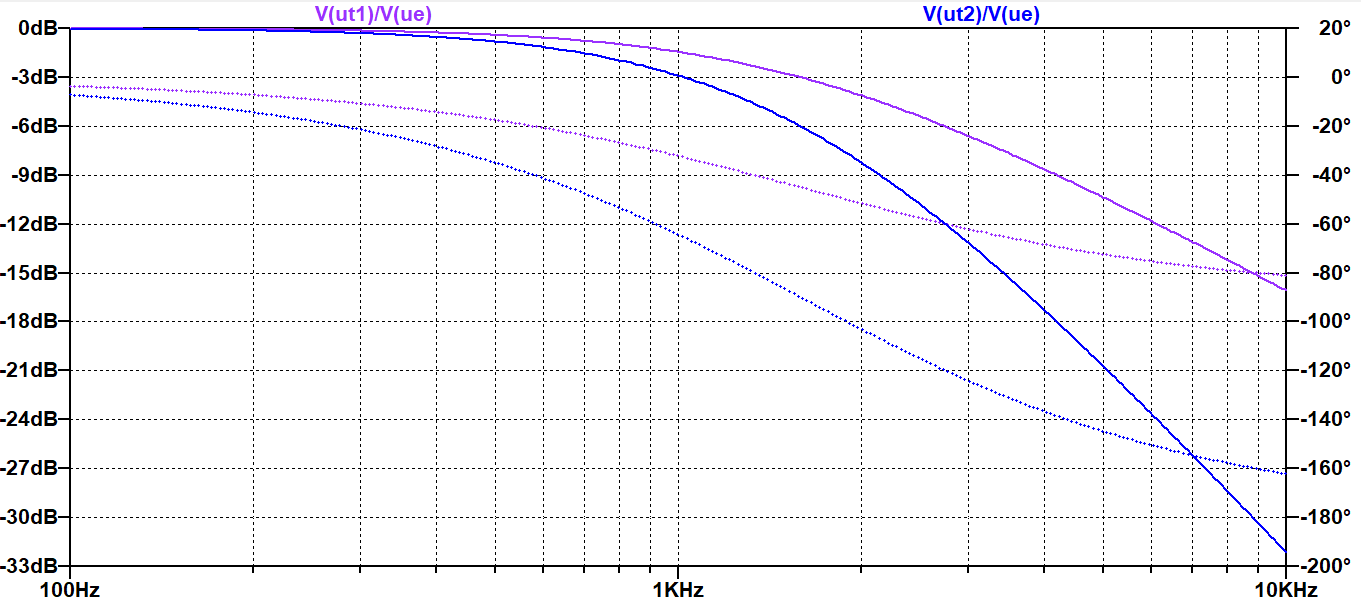
\includegraphics[width=16cm]{./pictures/Tiefpass_Bode}
    \caption{Bodediagram des Tiefpasses}
    \label{fig:TiefpassBode}
\end{figure}

\newpage

\begin{sidewaysfigure}[htb]
    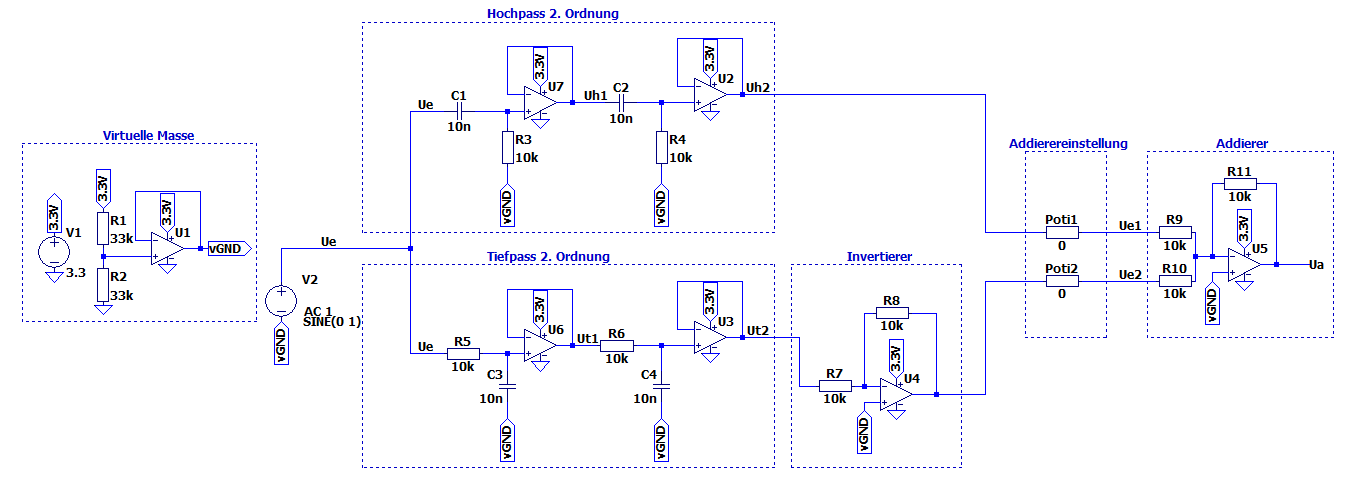
\includegraphics[width=24cm]{./pictures/Schaltung}
    \caption{Gesamtschaltung des Filters}
    \label{fig:Gesamtschaltung}
\end{sidewaysfigure}

\subsubsection{Ergebnisse}

\subsubsection{Diskussion}

\newpage
\subsection{Addierschaltung}

\subsubsection{Materialien \& Methoden}

\begin{figure}[htb]
    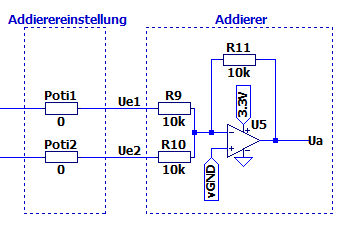
\includegraphics[width=16cm]{./pictures/Addierer}
    \caption{Addiererschaltung des Hoch- und Tiefpasses}
    \label{fig:Addierer}
\end{figure}

\begin{figure}[htb]
    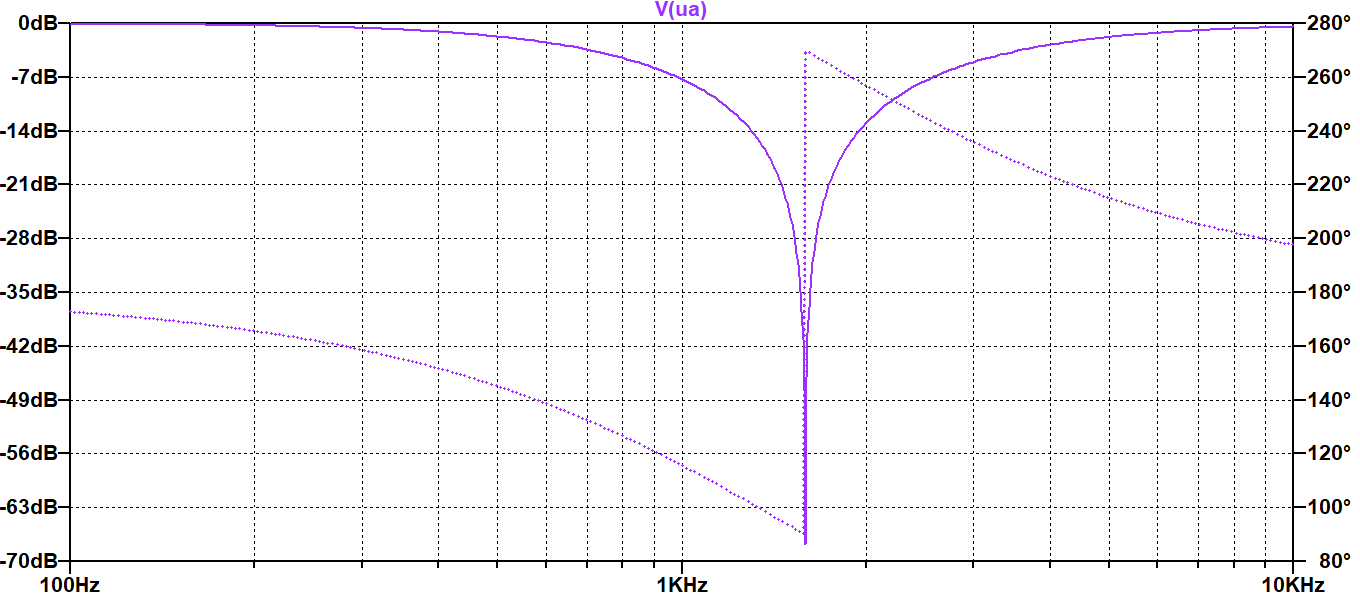
\includegraphics[width=16cm]{./pictures/Gesamtschaltung}
    \caption{Ausgangsspannung des Addierers}
    \label{fig:AddiererAusgangsspannung}
\end{figure}

\newpage
Die ermittelte Kurve zeigt, dass einer der Filter eine negative Spannung erzeugt. Nach weiteren Simulationen mit Spice wurde festgestellt, dass der Tiefpass negative Spannungen erzeugt. Aufgrund dessen muss das Ausgangssignal des Tiefpasses invertiert werden, da sonst die Ausgangssignale nicht addiert, sonst subtrahiert werden.

\begin{figure}[htb]
    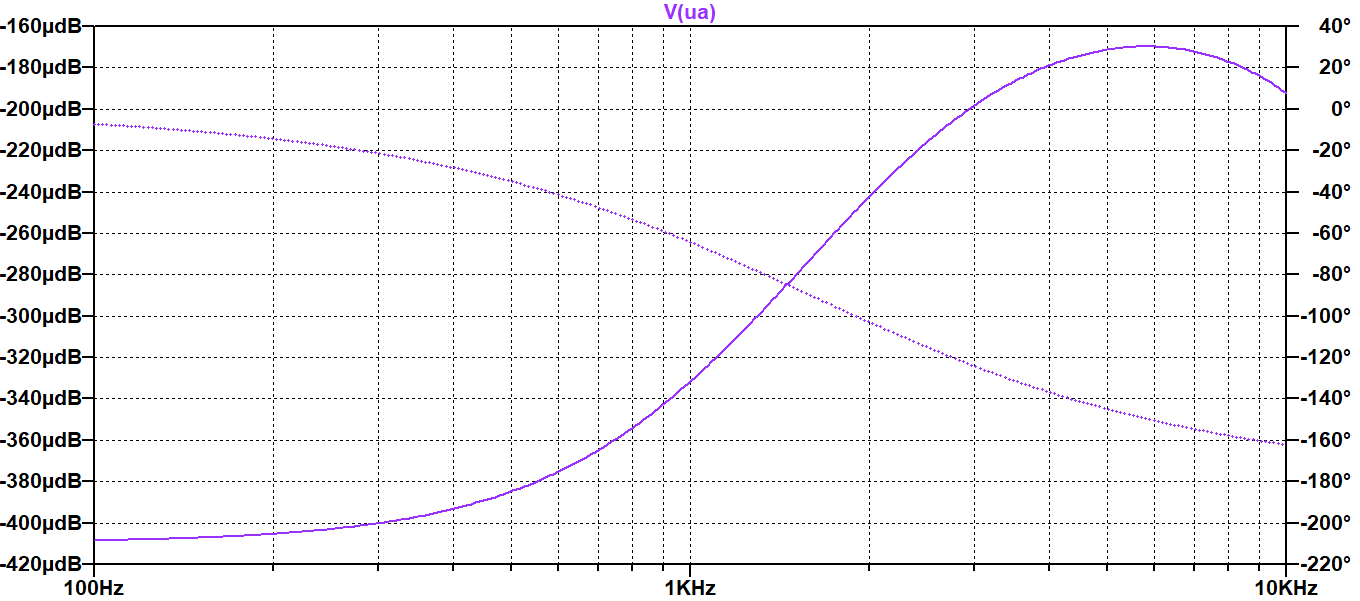
\includegraphics[width=16cm]{./pictures/Gesamtschaltung_Invertiert}
    \caption{Ausgangsspannung des Addierers mit invertiertem Tiefpass mit $R_1 = R_2 = 0$}
    \label{fig:AddiererAusgangsspannungInvertiert}
\end{figure}

Wir beobachten nun eine maximale Dämpfung des Signals bei 100Hz und Maximum bei ca 6000Hz. Die Funktion verläuft nun stetig ohne abrupte Änderung.
\\
\\
Einen solchen Filter bezeichnet man als 2-Band-Equalizer, da dieser aus einem kombinierten Hoch- und Tiefpass besteht und die jeweiligen Ausgangssignale des Hoch- und Tiefpasses einstellbar kombiniert werden können.

\begin{figure}[htb]
    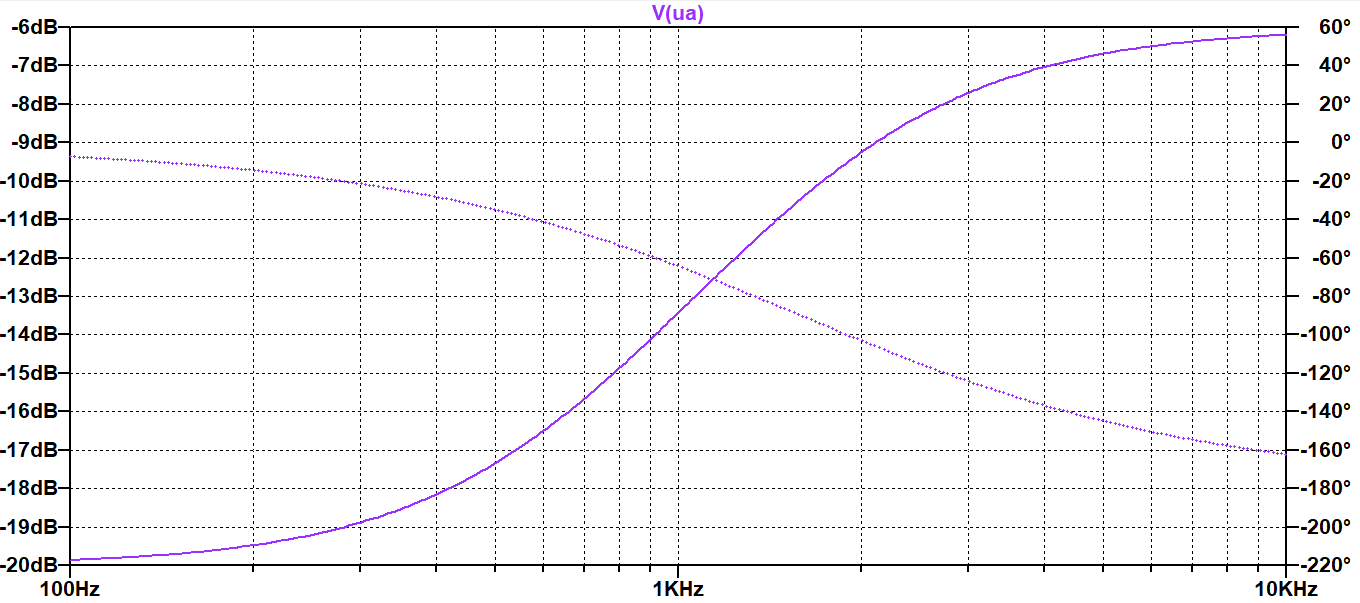
\includegraphics[width=16cm]{./pictures/Gesamtschaltung_Invertiert_10_90}
    \caption{Ausgangsspannung des Addierers mit invertiertem Tiefpass mit $R_1 = 10k\Omega$ und $R_2 = 90k\Omega$}
    \label{fig:AddiererAusgangsspannungInvertiert}
\end{figure}

\newpage
\begin{figure}[htb]
    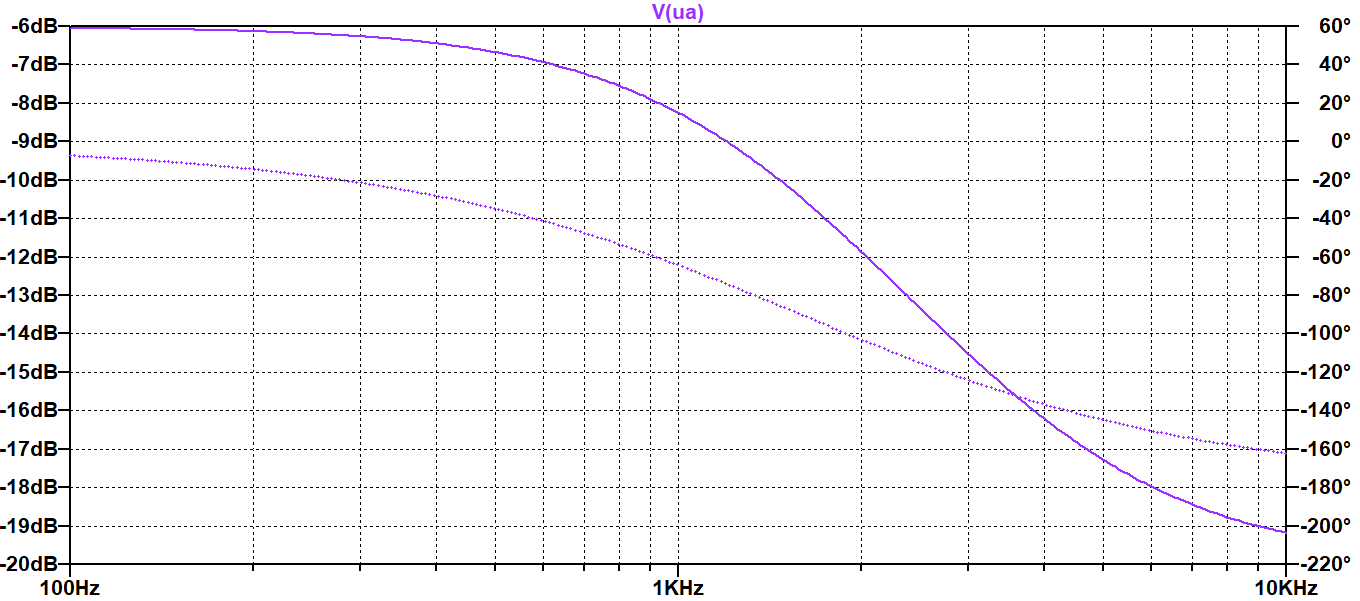
\includegraphics[width=16cm]{./pictures/Gesamtschaltung_Invertiert_90_10}
    \caption{Ausgangsspannung des Addierers mit invertiertem Tiefpass mit $R_1 = 90k\Omega$ und $R_2 = 10k\Omega$}
    \label{fig:AddiererAusgangsspannungInvertiert}
\end{figure}

Durch die Einstellungen an den Potentiometern lässt sich einstellen, welche Frequenzbereiche gedämpft werden sollen.
\subsubsection{Ergebnisse}

\subsubsection{Diskussion}
